\documentclass[11pt,a4paper]{article}

\usepackage[margin=2.25cm]{geometry}
\usepackage[T1]{fontenc}
\usepackage[utf8]{inputenc}
\usepackage{lmodern}
\usepackage{microtype}
\usepackage{amsmath,amssymb}
\usepackage{booktabs}
\usepackage{tabularx}
\usepackage{array}
\usepackage{graphicx}
\usepackage{float}
\usepackage{caption}
\usepackage{subcaption}
\usepackage{xcolor}
\usepackage{enumitem}
\usepackage{fancyhdr}
\usepackage{hyperref}
\usepackage{url}
\usepackage{pdflscape}
\usepackage{longtable}

\definecolor{navy}{HTML}{24445F}
\definecolor{blue}{HTML}{2F5D8A}
\definecolor{gold}{HTML}{D08C35}
\definecolor{purple}{HTML}{8B6AAE}
\definecolor{ink}{HTML}{30343B}
\definecolor{muted}{HTML}{5B6573}
\definecolor{rule}{HTML}{D9DEE5}
\definecolor{pale}{HTML}{F3F5F7}

\hypersetup{
  colorlinks=true,
  linkcolor=navy,
  citecolor=navy,
  urlcolor=blue,
  pdftitle={Cross-Market Momentum and Regime-Aware Protection},
  pdfsubject={Comparative evidence from US equities, MOEX equities, and Binance crypto},
  pdfauthor={Cross-Market Momentum Project}
}

\graphicspath{{generated/figures/}}
\setlength{\parindent}{0pt}
\setlength{\parskip}{0.55em}
\setlength{\emergencystretch}{2em}
\setlist[itemize]{leftmargin=1.5em,itemsep=0.25em,topsep=0.25em}
\setlist[enumerate]{leftmargin=1.7em,itemsep=0.25em,topsep=0.25em}
\captionsetup{font=small,labelfont=bf,labelsep=period}

\pagestyle{fancy}
\fancyhf{}
\fancyhead[L]{\footnotesize Cross-Market Momentum}
\fancyhead[R]{\footnotesize Frozen study through 2024}
\fancyfoot[C]{\thepage}
\renewcommand{\headrulewidth}{0.3pt}

\newcommand{\source}[1]{\par\vspace{0.15em}{\footnotesize\color{muted}\textit{Evidence source:} #1}}
\newcommand{\guardrail}[1]{%
  \begin{center}
  \fcolorbox{rule}{pale}{\begin{minipage}{0.93\linewidth}\small\textbf{Guardrail.} #1\end{minipage}}
  \end{center}
}
\newcommand{\resultbox}[1]{%
  \begin{center}
  \fcolorbox{navy}{pale}{\begin{minipage}{0.93\linewidth}\small #1\end{minipage}}
  \end{center}
}

\title{\vspace{-1.0cm}\textbf{Cross-Market Momentum and Regime-Aware Protection}\\[0.35em]
\large Comparative evidence from US equities, MOEX equities, and Binance crypto}
\author{Cross-Market Momentum Project\\\small Technical research report}
\date{Evidence frozen through 31 December 2024\\Report prepared July 2026}

\begin{document}

\maketitle

\begin{abstract}
This study tests whether a common cross-sectional momentum framework and a frozen volatility-based crash-protection overlay transfer across US equities, Russian equities, and Binance-traded cryptoassets. The experiment uses a unified monthly rebalanced, equal-weighted, market-neutral long-short construction; 27 momentum specifications per market; train-to-test walk-forward ranking; stability-gated finalist selection; market-specific transaction costs; and a chronological 2023--2024 retrospective holdout. The baseline grid shows a common medium-term region, especially the six-month lookback, but the corrected validation materially weakens the broad claim. MOEX provides the strongest, though still modest and regime-dependent, evidence: four configurations pass the frozen stability filter and the three-member ensemble earns 1.86\% annualized net return with a 0.26 Sharpe in the holdout. Crypto is mixed: two configurations pass the operational filter, the best single earns 2.36\% annualized, but the two-member ensemble loses 13.75\% annualized. The US control produces only one stable configuration, which loses 5.94\% annualized. The pre-specified 63-day/q90 volatility protection does not improve holdout performance consistently: it is inactive in crypto, effectively inactive in the US, and harmful to return, Sharpe, and maximum drawdown when active on MOEX. The principal finding is therefore conditional, not universal: medium-term momentum appears most transferable to MOEX in this sample, while volatility-based crash protection does not generalize out of validation.
\end{abstract}

\tableofcontents
\newpage

\section{Technical Summary}

\resultbox{\textbf{Main result.} A common medium-term momentum region is visible in the full baseline grid, but robust transfer is market-specific. The corrected train-to-test protocol finds modest positive evidence on MOEX, mixed evidence on crypto, and no positive holdout evidence in the US control. The tested regime-aware protection family does not produce a reliable cross-market improvement.}

The report answers the frozen Definition of Done questions as follows:

\begin{itemize}
  \item \textbf{MOEX momentum: moderate positive evidence.} Four of 24 eligible configurations are stable under the pre-specified filter. The frozen three-member ensemble earns 1.86\% annualized net with Sharpe 0.26 and maximum drawdown of -10.28\% in 2023--2024. The sign remains positive at 0, 10, and 20 bps transaction-cost assumptions.
  \item \textbf{Crypto momentum: mixed evidence, not family-level robustness.} Two of 27 configurations pass the operational stability filter, yet both fold-level rank correlations are negative. The best single earns 2.36\% annualized net, whereas the frozen two-member ensemble earns -13.75\% with Sharpe -0.62. Its failure is present even before transaction costs.
  \item \textbf{US momentum: weak transfer in the selected period.} Only one of 27 configurations is stable, so no stable ensemble is claimed. The frozen single earns -5.94\% annualized net with Sharpe -0.58.
  \item \textbf{Crash protection: no robust holdout benefit.} The frozen q90 rules do not activate in crypto, have no economically meaningful US intervention, and reduce MOEX performance when the portfolio-volatility rule is active. Attractive crisis-window behavior remains an in-sample diagnostic, not independent evidence.
\end{itemize}

\guardrail{Negative results are treated as research findings. No fold, stability threshold, finalist, transaction-cost assumption, volatility window, quantile, or logical protection rule is revised after observing the retrospective holdout.}

\section{Research Objective and Hypotheses}

The project asks whether the original Enhanced Momentum research framework transfers beyond its US-equity setting. The target outcome is not a production trading system or a general-purpose quant platform. It is a reproducible comparative answer to two questions:

\begin{enumerate}
  \item Does cross-sectional momentum remain economically positive and parameter-stable on MOEX equities and Binance cryptoassets under a common research design?
  \item Does a regime-aware volatility overlay reduce drawdown or tail loss without destroying the underlying strategy's return after costs?
\end{enumerate}

The hypotheses were directional rather than guaranteed: momentum could be weaker on the smaller, concentrated MOEX universe, stronger but more fragile in crypto, and crash protection could be more valuable in markets with abrupt regime changes. A null or negative result satisfies the project Definition of Done when it is produced without look-ahead, holdout selection, or post-hoc threshold changes.

The classical motivation is the persistence of winner-minus-loser returns documented in equities by Jegadeesh and Titman \cite{jegadeesh1993} and across markets and asset classes in later work \cite{rouwenhorst1998,asness2013}. The protection question follows evidence that momentum can experience episodic crashes, particularly around market rebounds and high-volatility states \cite{barroso2015,daniel2016}. This study does not assume those results must reproduce on MOEX or crypto; it tests transfer under a frozen implementation.

\section{Scope, Data, and Unified Contract}

\subsection{Market panels and investable universes}

The data layer exposes one market-agnostic contract: closing prices, daily returns, a volume or traded-value panel where available, a dynamic presence matrix, and a market proxy. The research engine consumes that contract rather than a source-specific schema.

\begin{table}[H]
\centering
\caption{Market data scope and primary transaction-cost assumptions. The full panels extend beyond some analysis windows; Phase 3 uses only dates specified by the frozen protocol.}
\resizebox{\textwidth}{!}{\footnotesize
\setlength{\tabcolsep}{5pt}
\begin{tabular}{llrrrr}
\toprule
Market & Source and universe & Panel span & Assets ever & Mean investable & Primary TC (bps) \\
\midrule
US & Supervisor Russell 3000 panel & 1979-12-31--2024-12-31 & 10593 & 1975.2 & 25 \\
MOEX & MOEX ISS, historical TQBR & 2013-03-25--2024-12-30 & 435 & 66.3 & 20 \\
Crypto & Binance Public Data, USDT pairs & 2018-01-01--2025-06-30 & 537 & 40.7 & 10 \\
\bottomrule
\end{tabular}
}
\source{Market YAML files and frozen data-quality reports in \texttt{backtests/enhanced\_momentum/reports/data\_quality}.}
\end{table}

\textbf{US equities.} The reference market uses the supervisor-provided Russell 3000-style panel. The data include 10,593 historical assets over the full archive and preserve inactive securities, which reduces simple end-of-sample survivorship bias. Volume is unavailable, and ordinary cash dividends are not included in the price-return strategy results.

\textbf{MOEX equities.} Daily data come from the MOEX ISS interface \cite{moexiss}. The loader discovers historical TQBR securities, including inactive names, and applies a lagged liquidity/presence rule. The panel contains 435 historical assets; the mean investable count is 66.3, but liquidity is concentrated, with the top ten assets representing 67\% of reported traded value in the data-quality report. MOEX prices are not treated as dividend-adjusted, and the 2022 market closure and sanctions episode is retained as a structural regime event.

\textbf{Crypto.} Daily 00:00 UTC candles come from Binance Public Data archives \cite{binancepublic}. The universe is a lagged-volume top-50 set of historically available USDT spot pairs, excluding stablecoins, leveraged tokens, and selected wrapped assets. The panel contains 537 assets, including 140 historical exits under the study's inactivity heuristic. It is therefore not restricted to current survivors, but it is also not a true historical top-50-by-market-cap universe.

\subsection{Data-quality facts that change interpretation}

The data are usable for a comparative study, but not homogeneous in quality:

\begin{itemize}
  \item MOEX has materially higher missingness within active lifetimes (mean 12.67\%) than crypto (0.01\%) and the US panel (5.43\%). The presence matrix and exact start/end price requirements are therefore important parts of the signal definition.
  \item The crypto panel has 602,648 pooled daily return observations, with a 99.9th percentile of +52.69\% and median asset annualized volatility of 130.4\%. Extreme returns are not automatically treated as errors.
  \item The MOEX universe is small in early years and has zero-investable-asset dates around market discontinuities. Three 12-month/zero-skip runs are retained for audit but excluded from finalist selection because a sparse observation caused a zero-target rebalance.
  \item US and MOEX results are price-return results. Excluding ordinary cash dividends can bias the relative performance of high-dividend shares and is especially relevant on MOEX.
\end{itemize}

\section{Momentum Methodology}

\subsection{Signal and portfolio construction}

At each month-end decision date $t$, the score for asset $i$ is the cumulative price return over a lookback of $L$ market observations, ending $S$ observations before the decision date:

\begin{equation}
  M_{i,t}(L,S) = \frac{P_{i,t-S}}{P_{i,t-S-L+1}} - 1.
\end{equation}

The eligible universe is restricted using the lagged presence matrix and requires exact asset-level prices at both signal endpoints. The highest-scoring fraction $q$ forms the long sleeve and the lowest-scoring fraction $q$ forms the short sleeve. Each sleeve is equal weighted and receives half of the total gross exposure:

\begin{equation}
  \sum_i |w_{i,t}| = 1, \qquad \sum_i w_{i,t}=0, \qquad
  \sum_{i:w_i>0}w_i=0.5, \quad \sum_{i:w_i<0}w_i=-0.5.
\end{equation}

Targets become effective on the next market observation, avoiding same-day signal execution. Between scheduled rebalances, weights drift within fixed-notional long and short sleeves and each sleeve is renormalized independently. A temporarily missing held price is marked at the last observation, creating zero return while stale and recognizing the accumulated price change when a new close appears.

One-way turnover is defined as half the $L^1$ target-weight change. For cost $c_m$ basis points in market $m$, the reconstructed net return is

\begin{equation}
  r^{\mathrm{net}}_{t,m}=r^{\mathrm{gross}}_{t,m}-\mathrm{turnover}_{t,m}\frac{c_m}{10{,}000},
\end{equation}

with primary costs of 25 bps for US, 20 bps for MOEX, and 10 bps for crypto. These costs capture a stylized trading drag, not financing, borrow availability, funding rates, or nonlinear market impact.

\subsection{Frozen baseline grid}

Each market has 27 configurations: three lookbacks, three skips, and three tail quantiles. US and MOEX use 126/252/504-observation lookbacks and 0/21/63-observation skips; crypto uses 182/365/730 observations and 0/30/91-observation skips. Tail fractions are 10\%, 20\%, and 30\%. The common evaluation start within each market is chosen so every configuration has enough history, preventing shorter lookbacks from receiving a longer evaluation sample.

\subsection{Metrics and comparison basis}

Returns are annualized with 252 observations for US and MOEX and 365 for crypto. Sharpe is the annualized mean-to-volatility ratio with a zero risk-free rate. Maximum drawdown is the minimum of $NAV_t/\max_{s\le t}NAV_s-1$. The Information Ratio against SPX, IMOEX, or BTC is reported descriptively but not used to select configurations: the strategy is market neutral while each proxy is long only, so the two quantities answer different economic questions.

\section{Baseline Grid: A Common Six-Month Region, but Not a Final Claim}

The 81-run gross baseline shows the same broad horizon pattern in all three markets: the six-month lookback is strongest on average, the 12-month horizon is weaker, and the 24-month horizon deteriorates. That pattern is useful for describing the parameter surface, but it is not sufficient evidence of transfer because it uses the full baseline history and does not test train-to-test selection.

\begin{figure}[H]
\centering
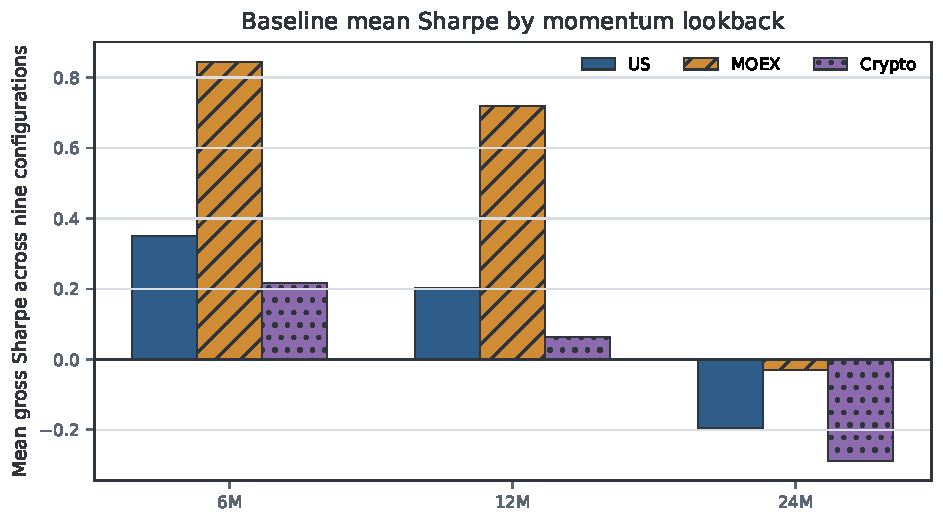
\includegraphics[width=0.88\textwidth]{baseline_lookback.pdf}
\caption{Mean gross Sharpe by lookback. Each bar averages nine skip/quantile configurations. MOEX is strongest in the baseline grid; the 24-month horizon is negative on average in all three markets.}
\source{\texttt{results/baseline\_grid\_v5/final\_analysis/table\_lookback\_effect.csv}.}
\end{figure}

\begin{table}[H]
\centering
\caption{Full-history gross baseline overview. These results describe the grid and are not used as final holdout evidence.}
\resizebox{\textwidth}{!}{\footnotesize
\setlength{\tabcolsep}{5pt}
\begin{tabular}{lrrlrrr}
\toprule
Market & Positive Sharpe & Mean Sharpe & Best configuration & Best Sharpe & Best ann. return & Best MaxDD \\
\midrule
US & 18/27 & 0.118 & us\_lb6M\_sk3M\_q10 & 0.489 & 4.50\% & -42.8\% \\
MOEX & 22/27 & 0.511 & moex\_lb6M\_sk0M\_q30 & 1.050 & 7.96\% & -20.0\% \\
Crypto & 15/27 & -0.002 & crypto\_lb6M\_sk1M\_q20 & 0.573 & 13.90\% & -31.1\% \\
\bottomrule
\end{tabular}
}
\source{Frozen baseline grid v5 final-analysis tables.}
\end{table}

The cleanest common baseline region is 6M/1M with 20--30\% tails. The 6M/1M/20\% specification has positive Sharpe in all three markets, mean Sharpe 0.604, and worst-market Sharpe 0.368. However, the corrected Phase 3 protocol deliberately does not promote that full-history observation into a universal rule. Configurations must first show transfer from past train windows to subsequent test windows.

\section{Corrected Walk-Forward Design and Frozen Selection}

\subsection{Why the protocol was amended}

The provisional Phase 3 analysis ranked configurations across separate validation periods but did not implement a complete train-to-test ranking within every fold. It also forced three-member ensembles. Before rerunning the analysis, the project recorded a protocol amendment that preserved the 81 frozen baseline return series but replaced the selection layer with an explicit walk-forward design.

For every fold, all eligible configurations are ranked by primary-cost net Sharpe on the train window and independently ranked on the subsequent test window. All configurations share a common date index inside each sample. The final 2023--2024 interval is excluded from algorithmic selection.

\guardrail{Because full-sample baseline summaries through 2024 had already been inspected before the amendment, 2023--2024 is called a chronological retrospective holdout or pseudo-OOS. It is not represented as a pristine untouched OOS sample.}

\subsection{Operational definition of a stable configuration}

With 27 configurations, the top third is ranks 1--9; with 24 eligible MOEX configurations, it is ranks 1--8. A configuration is stable only if all five frozen criteria hold:

\begin{enumerate}
  \item median train rank is in the top third;
  \item median test rank is in the top third;
  \item test top-third membership occurs in at least 50\% of folds;
  \item test net Sharpe is positive in at least 50\% of folds; and
  \item median absolute train-to-test rank change is no greater than one top-third width.
\end{enumerate}

This is an operational parameter-transfer rule, not a statistical test of alpha. Ensemble size is also frozen: three or more stable configurations permit an ens-3, exactly two permit an ens-2, and fewer than two produce no stable ensemble. No unstable member can be added to fill a slot. Candidate return correlation is capped at 0.95 when assembling the ensemble.

\subsection{Rank transfer is uneven and weakest in crypto}

\begin{figure}[H]
\centering
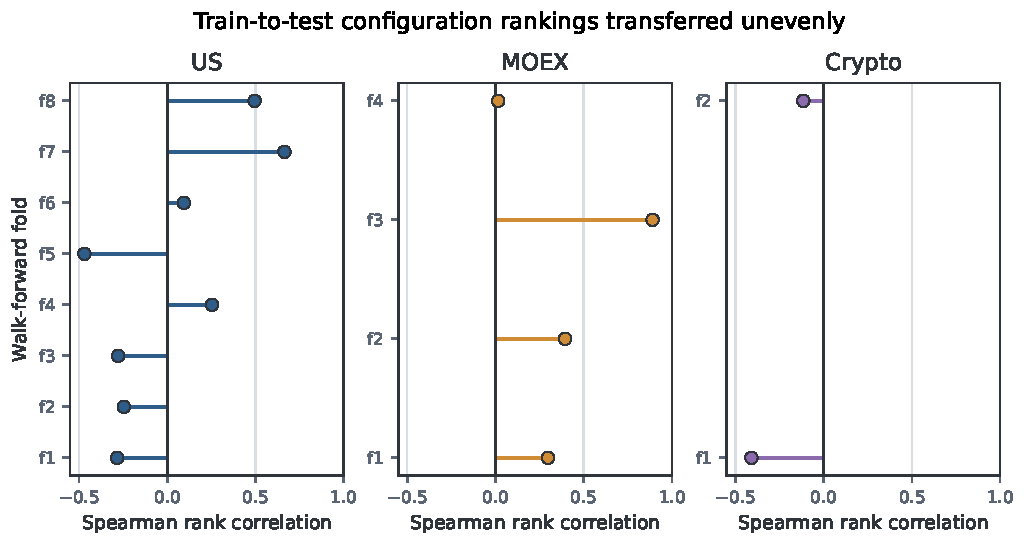
\includegraphics[width=0.95\textwidth]{rank_transfer.pdf}
\caption{Spearman correlation between train and subsequent test ranks. Negative values mean that strong train rankings tended to reverse in the next test period. Crypto is negative in both folds; MOEX contains one strong-transfer fold but also a near-zero final fold; US varies substantially over time.}
\source{\texttt{results/phase3/fold\_rank\_stability.csv}.}
\end{figure}

Crypto has train-to-test Spearman correlations of -0.410 and -0.115, with only 11.1\% retention of train top-third configurations in each test fold. MOEX is more favorable but heterogeneous: correlations are 0.297, 0.395, 0.890, and 0.016. US has five negative or near-zero early fold correlations before stronger positive transfer in 2021 and 2022. Consequently, the existence of a few stable configurations must not be confused with stability of the entire ranking surface.

\begin{table}[H]
\centering
\caption{Frozen finalist selection. Ensemble members are selected only from the stable set.}
\resizebox{\textwidth}{!}{\scriptsize
\setlength{\tabcolsep}{5pt}
\begin{tabular}{lrrlll}
\toprule
Market & Eligible & Stable & Best frozen single & Ensemble & Members \\
\midrule
US & 27 & 1 & us\_lb6M\_sk1M\_q10 & no\_stable\_ensemble & none \\
MOEX & 24 & 4 & moex\_lb6M\_sk1M\_q30 & ens3 & moex\_lb6M\_sk1M\_q30, moex\_lb6M\_sk3M\_q20, moex\_lb6M\_sk1M\_q20 \\
Crypto & 27 & 2 & crypto\_lb6M\_sk1M\_q30 & ens2 & crypto\_lb6M\_sk1M\_q30, crypto\_lb12M\_sk3M\_q20 \\
\bottomrule
\end{tabular}
}
\source{\texttt{results/phase3/config\_stability.csv}, \texttt{finalist\_selection\_audit.csv}, and \texttt{frozen\_selection.json}.}
\end{table}

US produces one stable configuration and therefore no stable ensemble. MOEX produces four stable configurations and an ens-3 of closely related six-month specifications. Crypto produces two stable configurations and an ens-2, even though its market-level ranking transfer is poor. That tension is preserved as a finding rather than resolved by changing the stability criteria after the result is known.

\section{Retrospective Holdout: MOEX Is Positive, Crypto Is Mixed, US Is Negative}

\subsection{Frozen portfolio results}

\begin{figure}[H]
\centering
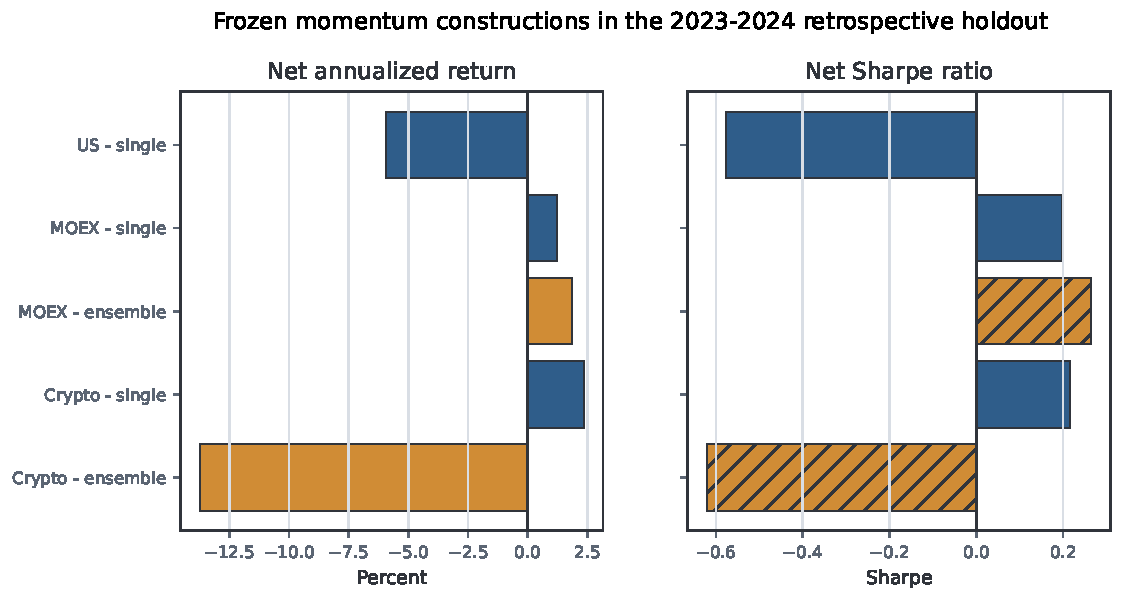
\includegraphics[width=0.93\textwidth]{holdout_performance.pdf}
\caption{Net performance of frozen momentum constructions in the 2023--2024 retrospective holdout. The MOEX single and ensemble remain positive; the crypto single is slightly positive but the stable ensemble is negative; the US single is negative.}
\source{\texttt{results/phase3/benchmark\_comparison.csv}. Primary costs: US 25 bps, MOEX 20 bps, crypto 10 bps.}
\end{figure}

\begin{table}[H]
\centering
\caption{Retrospective holdout comparison. Market proxies are long-only context, not substitutes for the market-neutral momentum portfolios.}
\resizebox{\textwidth}{!}{\footnotesize
\setlength{\tabcolsep}{5pt}
\begin{tabular}{llrrrrr}
\toprule
Market & Portfolio & Ann. return & Ann. vol & Sharpe & MaxDD & Corr. to proxy \\
\midrule
US & Market proxy & 25.8\% & 12.9\% & 1.85 & -9.9\% & 1.00 \\
US & Best frozen single & -5.9\% & 9.8\% & -0.58 & -13.9\% & -0.11 \\
MOEX & Market proxy & 15.5\% & 17.9\% & 0.89 & -32.1\% & 1.00 \\
MOEX & Best frozen single & 1.2\% & 7.6\% & 0.20 & -9.3\% & -0.15 \\
MOEX & Stable ensemble & 1.9\% & 8.3\% & 0.26 & -10.3\% & -0.10 \\
Crypto & Market proxy & 137.6\% & 48.8\% & 2.02 & -26.2\% & 1.00 \\
Crypto & Best frozen single & 2.4\% & 23.4\% & 0.22 & -23.4\% & 0.08 \\
Crypto & Stable ensemble & -13.7\% & 20.5\% & -0.62 & -29.1\% & 0.04 \\
\bottomrule
\end{tabular}
}
\source{\texttt{results/phase3/benchmark\_comparison.csv}.}
\end{table}

\textbf{MOEX gives the strongest transfer evidence, but the economic magnitude is small.} The best frozen single earns 1.22\% annualized net with Sharpe 0.20 and maximum drawdown -9.28\%. The ens-3 improves annualized return to 1.86\% and Sharpe to 0.26, with maximum drawdown -10.28\%. Four stable configurations and a positive net ensemble support a moderate claim, not a universal one, because the fold-level rank transfer is inconsistent and dividends are excluded.

\textbf{Crypto does not support a broad family-level momentum claim.} The best single earns 2.36\% annualized with Sharpe 0.22, but the ens-2 loses 13.75\% annualized with Sharpe -0.62 and maximum drawdown -29.15\%. The result shows that two configurations can satisfy a coarse operational stability filter while their equal-weight combination fails in the next regime. It is therefore more accurate to say that a single specification shows weak transfer than to claim that crypto momentum is robust.

\textbf{The US control is negative in this holdout.} The only stable configuration loses 5.94\% annualized with Sharpe -0.58 and maximum drawdown -13.88\%. This does not refute the historical momentum literature; it shows that the frozen specification family and selected period do not produce positive transfer in this implementation.

\begin{figure}[H]
\centering
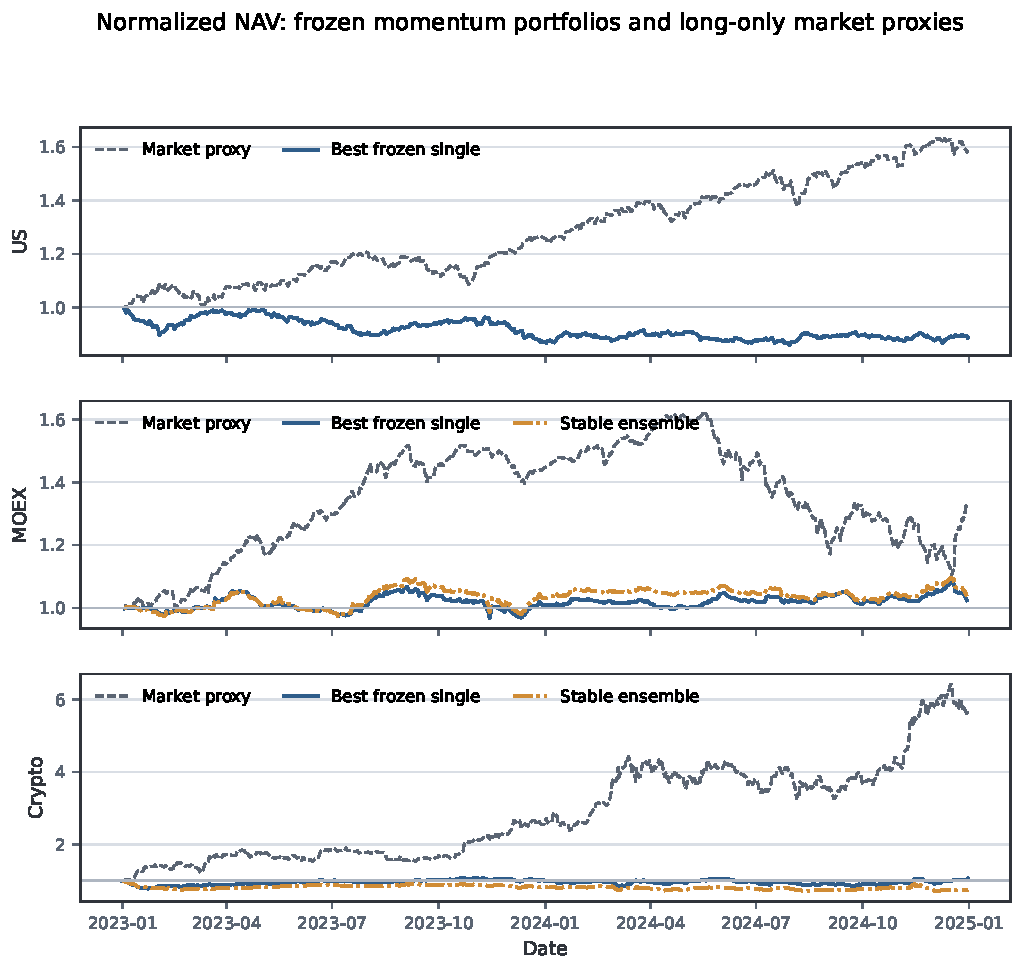
\includegraphics[width=0.92\textwidth]{holdout_nav.pdf}
\caption{Normalized NAV for momentum portfolios and market proxies. The proxy paths provide regime context only: comparing a market-neutral long-short factor directly with a long-only index is not an investable replacement test.}
\source{\texttt{results/phase3/oos\_nav.parquet}.}
\end{figure}

The long-only proxies rally strongly in 2023--2024, especially BTC. Momentum correlations to the proxies are small: -0.10 to -0.15 for the MOEX constructions, 0.04--0.08 for crypto, and -0.11 for the US single. Negative proxy-relative Information Ratios therefore mainly reflect a different exposure objective and are not the primary momentum-premium criterion.

\section{Transaction Costs Do Not Explain the Main Signs}

Primary-cost selection is not rerun at alternative costs. The already frozen best single and base construction are evaluated mechanically under pre-specified scenarios.

\begin{figure}[H]
\centering
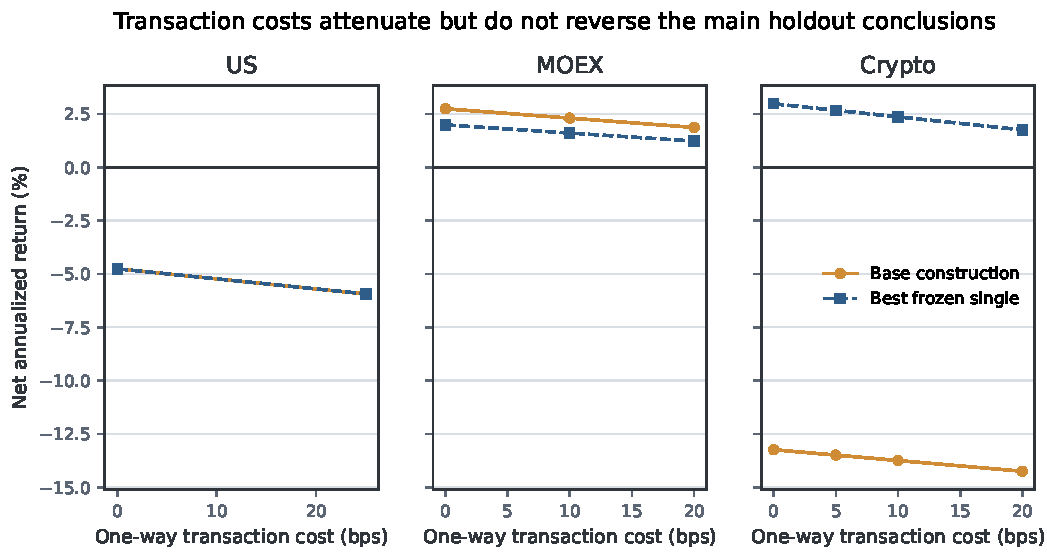
\includegraphics[width=0.95\textwidth]{tc_sensitivity.pdf}
\caption{Net annualized return under pre-specified one-way transaction-cost scenarios. Higher costs reduce returns monotonically, but the core signs remain: MOEX stays positive, the crypto ensemble stays negative, and the US single is negative even at zero cost.}
\source{\texttt{results/phase3/tc\_sensitivity.csv}; retrospective holdout rows only.}
\end{figure}

MOEX ens-3 annualized return declines from 2.74\% at zero cost to 2.30\% at 10 bps and 1.86\% at 20 bps. The crypto best single stays positive from 2.97\% at zero cost to 1.75\% at 20 bps, whereas the ens-2 is negative even at zero cost (-13.24\%). The US single is also negative before costs (-4.76\%) and falls to -5.94\% at 25 bps. Thus, costs attenuate performance but do not create the principal cross-market conclusions.

\section{Regime-Aware Protection}

\subsection{Frozen design}

Protection is applied to the final base construction for each market: the US stable single, MOEX ens-3, and crypto ens-2. Two features are computed continuously through the validation/holdout boundary:

\begin{align}
  \sigma^{p}_{t} &= \operatorname{Std}_{63}(r^{p})_{t-1}, \\
  \sigma^{m}_{t} &= \operatorname{Std}_{63}(r^{m})_{t-1}.
\end{align}

The one-observation shift prevents the current return from entering the current exposure decision. The 90th-percentile thresholds are calibrated only on pre-holdout history and frozen. Four rules are retained: no protection, portfolio-volatility q90, market-volatility q90, and the logical AND of both signals. Risk-off exposure is zero; normal exposure is one. Each exposure switch incurs incremental half-$L^1$ turnover at the market's primary cost.

No protection variant is selected using holdout performance. A rule that does not fire, fires too often, or worsens performance is an admissible negative result.

\subsection{Holdout protection is inactive or harmful}

\begin{figure}[H]
\centering
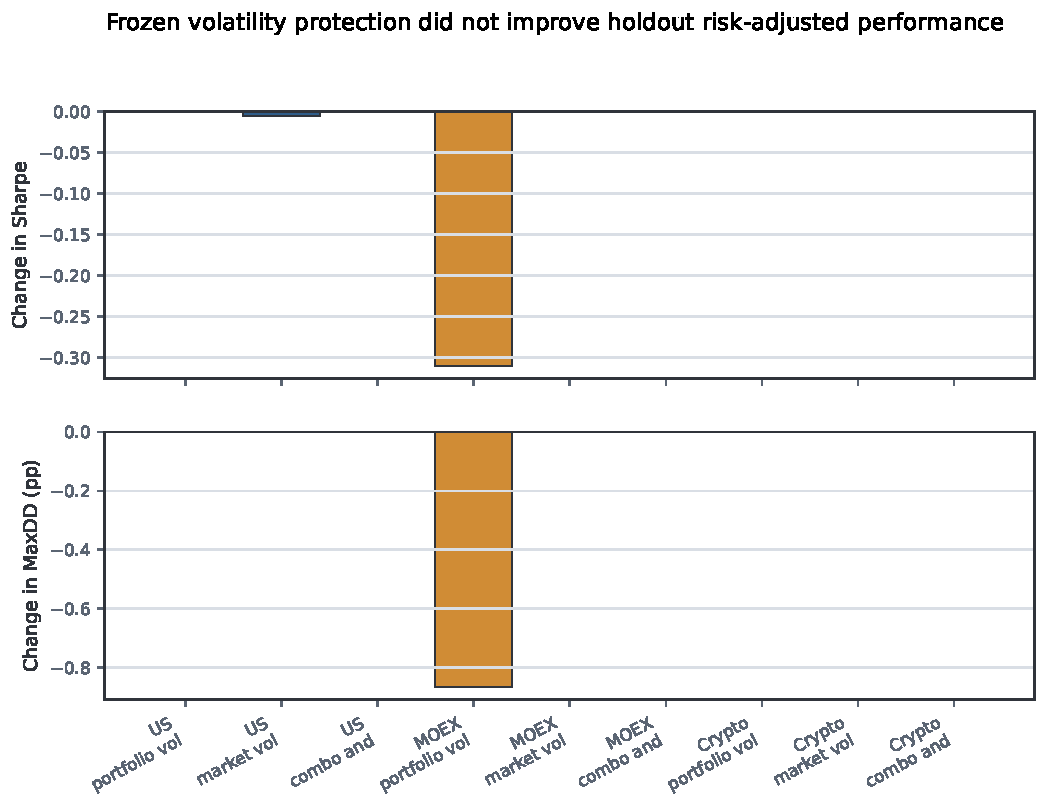
\includegraphics[width=0.94\textwidth]{protection_effects.pdf}
\caption{Changes relative to no protection in the retrospective holdout. Positive change in maximum drawdown means a shallower drawdown. Most rules are inactive; the active MOEX portfolio-volatility rule reduces Sharpe and makes maximum drawdown slightly worse.}
\source{\texttt{results/phase3/protection/protection\_results.csv}.}
\end{figure}

\begin{table}[H]
\centering
\caption{Frozen protection outcomes relative to no protection. Zero values generally indicate that the rule did not fire.}
\resizebox{\textwidth}{!}{\scriptsize
\setlength{\tabcolsep}{5pt}
\begin{tabular}{llrrrrr}
\toprule
Market & Rule & Risk-off & Switches & $\Delta$ ann. return & $\Delta$ Sharpe & $\Delta$ MaxDD \\
\midrule
US & portfolio\_vol\_q90 & 0.0\% & 0 & 0.00\% & 0.00 & 0.00 pp \\
US & market\_vol\_q90 & 0.0\% & 1 & -0.06\% & -0.01 & -0.00 pp \\
US & combo\_and\_q90 & 0.0\% & 0 & 0.00\% & 0.00 & 0.00 pp \\
MOEX & portfolio\_vol\_q90 & 19.4\% & 4 & -2.42\% & -0.31 & -0.87 pp \\
MOEX & market\_vol\_q90 & 0.0\% & 0 & 0.00\% & 0.00 & 0.00 pp \\
MOEX & combo\_and\_q90 & 0.0\% & 0 & 0.00\% & 0.00 & 0.00 pp \\
Crypto & portfolio\_vol\_q90 & 0.0\% & 0 & 0.00\% & 0.00 & 0.00 pp \\
Crypto & market\_vol\_q90 & 0.0\% & 0 & 0.00\% & 0.00 & 0.00 pp \\
Crypto & combo\_and\_q90 & 0.0\% & 0 & 0.00\% & 0.00 & 0.00 pp \\
\bottomrule
\end{tabular}
}
\source{\texttt{results/phase3/protection/protection\_results.csv} and \texttt{signal\_diagnostics.csv}.}
\end{table}

\textbf{Crypto.} Neither feature exceeds its frozen threshold in 2023--2024. Portfolio-volatility peaks at 1.83\% daily versus a 2.04\% threshold; market-volatility peaks at 3.61\% versus 4.88\%. Every protection variant is therefore identical to the -13.75\% annualized base. The negative premium is a prolonged adverse momentum regime, not a high-volatility crash under the tested feature family.

\textbf{US.} Portfolio-volatility and AND never fire. The market-volatility rule has no in-holdout risk-off days, but one boundary state transition produces 0.125\% arithmetic switching drag and a small performance deterioration. This is not evidence of protection effectiveness.

\textbf{MOEX.} Market-volatility and AND do not fire. Portfolio-volatility is risk-off 19.41\% of the holdout and switches four times. Annualized return falls from 1.86\% to -0.56\%, Sharpe falls from 0.26 to -0.05, and maximum drawdown worsens from -10.28\% to -11.15\%. Expected shortfall at the 1\% level improves only marginally, from -1.979\% to -1.946\% per day. The overlay sacrifices exposure and pays switching costs without improving the main risk metrics.

\subsection{Crisis windows explain the mechanism but are not OOS evidence}

The validation crisis diagnostics show why the idea was plausible. In the US COVID window, market-volatility protection reduced maximum drawdown from -5.82\% to -0.30\%. During the 2022 MOEX structural-break window, portfolio-volatility protection reduced maximum drawdown from -14.39\% to -5.60\%. In the 2021 crypto selloff, market-volatility protection improved total return, while portfolio-volatility protection reduced drawdown but worsened total return. In the 2022 crypto crisis, none of the q90 signals fired.

These episodes are explicitly labeled \texttt{in\_sample\_validation\_diagnostic\_only}. Their attractive cases do not override the holdout result. The contrast is itself informative: a protection rule can look useful in named historical crises yet fail to transfer because later losses occur below its calibrated volatility threshold or because it exits during recoveries.

\section{Cross-Market Interpretation}

\subsection{Where momentum works and where it does not}

\textbf{MOEX: modest reproducibility.} The combination of four stable configurations, a positive ens-3, and persistence under transaction costs provides the strongest support. Plausible contributors include slower information diffusion and pronounced medium-term regimes. Countervailing forces remain material: small effective cross-sections, sector concentration, dividend gaps, missing prices, and the 2022 structural break.

\textbf{Crypto: isolated transfer without ensemble robustness.} The baseline six-month region is positive, and one frozen single remains slightly profitable after costs. Yet the ranking surface reverses across both walk-forward folds and the ens-2 fails before costs. Strong trends at the asset level do not automatically imply a stable cross-sectional winner-minus-loser premium once listing dynamics, regime changes, and equal-weight ensemble construction are imposed.

\textbf{US: a useful negative control.} The baseline contains many positive gross configurations, but the corrected transfer test leaves one stable single and a negative holdout. This demonstrates why a favorable full-history grid should not be equated with a deployable frozen selection.

\subsection{Why protection does not generalize}

The tested overlay protects only against a narrow state definition: lagged 63-observation volatility above a pre-holdout 90th percentile. Momentum can lose through other mechanisms, including slow factor decay, leadership reversal without unusually high volatility, or repeated modest losses. Crypto provides the clearest counterexample: the ens-2 loses materially while both volatility features remain below threshold throughout the holdout.

The result does not show that all dynamic risk management is useless. It shows that this fixed volatility-only family, calibrated as specified, does not transfer reliably across these markets and periods. Testing other features or thresholds would constitute future research and must begin with a new pre-registered holdout rather than a post-hoc repair of the current result.

\section{Limitations and Threats to Validity}

\begin{enumerate}
  \item \textbf{Retrospective rather than pristine holdout.} Selection code excludes 2023--2024, but full-sample baseline summaries through 2024 were viewed before the corrected protocol. Claims are therefore descriptive and retrospective.
  \item \textbf{No statistical multiple-testing correction.} The project controls data snooping operationally through frozen grids, walk-forward transfer, stability gating, and a holdout, but it does not report deflated Sharpe ratios, SPA tests, or family-wise error corrections. A stable configuration is not equivalent to statistically significant alpha.
  \item \textbf{Price returns and corporate actions.} Ordinary cash dividends are excluded for US and MOEX. MOEX split/corporate-action handling and sparse sessions can distort price momentum; three known sparse-signal runs are excluded from selection but retained in audit outputs.
  \item \textbf{Universe definitions differ.} US approximates a broad Russell 3000-style panel, MOEX uses historical TQBR with lagged liquidity, and crypto uses Binance-tradable top-lagged-volume pairs rather than a historical market-cap universe. Cross-market comparison is methodological, not a perfectly matched natural experiment.
  \item \textbf{Crypto fold count is low.} Only two pre-holdout folds are available, so configuration-level stability is directionally informative and statistically weak.
  \item \textbf{Implementation costs are incomplete.} Linear transaction costs exclude bid-ask nonlinearity, market impact, short borrow fees and availability, margin, funding rates, exchange constraints, taxes, and capital controls. A market-neutral crypto portfolio is a factor simulation, not a directly executable Binance spot strategy.
  \item \textbf{Shorting and market access.} MOEX and crypto short legs may be difficult or impossible to implement at reported prices. The results identify a return pattern, not a certified tradable product.
  \item \textbf{Benchmark mismatch.} SPX, IMOEX, and BTC are long-only proxies, while the strategy targets zero net exposure. Proxy-relative Information Ratios are contextual, not selection objectives.
  \item \textbf{Regime family is narrow.} Only lagged 63-observation portfolio/market volatility, q90 thresholds, and the AND combination are tested. A non-firing rule is a design limitation and a valid result, not a justification for holdout retuning.
  \item \textbf{Structural breaks and evolving venues.} MOEX 2022 and the rapidly changing Binance listing environment may violate the assumption that pre-holdout relationships remain stable.
\end{enumerate}

\section{Conclusions}

The study achieves its central objective: it applies one auditable momentum and crash-protection framework to three distinct markets and reports where the evidence transfers and where it fails.

\begin{itemize}
  \item \textbf{Momentum is not universal under a frozen specification family.} The six-month region is common in the gross baseline, but corrected walk-forward and holdout evidence differ sharply by market.
  \item \textbf{MOEX provides the best, still modest, evidence.} Its stable ens-3 remains positive after 20 bps costs, although the annualized return is only 1.86\% and the rank-transfer record is uneven.
  \item \textbf{Crypto does not support robust ensemble transfer.} A best single is weakly positive, but negative fold-level rank correlations and a losing ens-2 argue against a broad premium claim.
  \item \textbf{The US control is negative in 2023--2024.} This reinforces the need to distinguish a historically favorable parameter surface from forward transfer.
  \item \textbf{Volatility-based crash protection is not portable in this experiment.} It is inactive where crypto and US momentum are weak and harmful where it activates on MOEX. Validation crisis gains do not generalize to the retrospective holdout.
\end{itemize}

The honest final statement is therefore:

\resultbox{Cross-sectional momentum shows moderate, regime-dependent reproducibility on MOEX; only isolated and unstable evidence on Binance crypto; and no positive transfer in the US control holdout. The frozen 63-day/q90 regime-aware protection does not improve results consistently across markets and cannot be presented as a universal crash solution.}

\section{Recommended Next Steps and Open Questions}

The current experiment should remain frozen. Future work should start a new protocol and a new genuinely unseen evaluation period. The highest-value extensions are:

\begin{enumerate}
  \item construct dividend-adjusted or total-return equity series, especially for MOEX;
  \item obtain a true historical crypto market-cap universe and delisting-aware return treatment;
  \item model borrow, funding, bid-ask spread, and nonlinear impact explicitly;
  \item pre-register a new protection family based on drawdown state, correlation dispersion, or trend breaks, with no reuse of 2023--2024 for selection;
  \item evaluate whether ensemble weighting should reward cross-fold covariance stability rather than equal weighting; and
  \item add multiple-testing-aware inference and confidence intervals while preserving the current frozen results as a separate research generation.
\end{enumerate}

Open questions include whether MOEX's positive result survives total-return adjustment, whether crypto's losing ensemble is specific to the 2023--2024 leadership regime, and whether a crash-protection signal can distinguish abrupt volatility shocks from slow momentum decay.

\appendix

\section{Frozen Walk-Forward Folds}

\begin{table}[H]
\centering
\caption{Pre-holdout train/test windows in the corrected Phase 3 protocol. Actual common starts may be later when required by shared data availability.}
\scriptsize
\setlength{\tabcolsep}{5pt}
\begin{tabular}{llll}
\toprule
Market & Fold & Train & Test \\
\midrule
US & us\_f1 & 2010--2014 & 2015--2015 \\
US & us\_f2 & 2010--2015 & 2016--2016 \\
US & us\_f3 & 2010--2016 & 2017--2017 \\
US & us\_f4 & 2010--2017 & 2018--2018 \\
US & us\_f5 & 2010--2018 & 2019--2019 \\
US & us\_f6 & 2010--2019 & 2020--2020 \\
US & us\_f7 & 2010--2020 & 2021--2021 \\
US & us\_f8 & 2010--2021 & 2022--2022 \\
MOEX & moex\_f1 & 2013--2016 & 2017--2018 \\
MOEX & moex\_f2 & 2013--2018 & 2019--2020 \\
MOEX & moex\_f3 & 2013--2020 & 2021--2021 \\
MOEX & moex\_f4 & 2013--2021 & 2022--2022 \\
Crypto & crypto\_f1 & 2018--2020 & 2021--2021 \\
Crypto & crypto\_f2 & 2019--2021 & 2022--2022 \\
\bottomrule
\end{tabular}

\source{\texttt{config/phase3\_protocol\_v2.yaml}.}
\end{table}

\section{Reproducibility}

The report is generated only from frozen repository artifacts. From the repository root:

\begin{verbatim}
source .venv/bin/activate
MPLCONFIGDIR=/tmp/cmm-mpl python reports/final/build_report_assets.py
cd reports/final
tectonic cross_market_momentum_report.tex
\end{verbatim}

The first command recreates all report tables and vector figures and validates the expected evidence shape: 81 baseline runs, 14 walk-forward folds, seven stable configurations, the 2023--2024 holdout envelope, four frozen protection variants, and crisis rows labeled as validation diagnostics. It also writes \texttt{generated/source\_manifest.csv} with SHA-256 hashes for every material local source.

The analytical pipeline itself is reproduced from the project root with the frozen baseline and Phase 3 runners. The report does not rerun the 81 baseline backtests; Phase 3 intentionally consumes the saved daily returns and turnover files from \texttt{results/baseline\_grid\_v5/runs}.

\section{Guardrail Checklist}

\begin{itemize}
  \item Baseline grid and underlying daily series remain frozen.
  \item Train ranks are computed only on past windows; test ranks use the subsequent fold.
  \item Stable-config rules are defined before the corrected holdout run.
  \item No unstable configuration is added to force an ensemble.
  \item Primary selection uses net Sharpe at pre-specified market costs.
  \item Alternative cost levels are sensitivity checks, not new selection loops.
  \item Protection thresholds are calibrated only on pre-holdout history and shifted by one observation.
  \item No q80/q85, different window, OR rule, or holdout-winning variant is introduced after results are observed.
  \item Named crisis windows are validation diagnostics only.
  \item Negative results remain visible and are not replaced by post-hoc specifications.
\end{itemize}

\begin{thebibliography}{99}

\bibitem{jegadeesh1993}
N. Jegadeesh and S. Titman.
Returns to Buying Winners and Selling Losers: Implications for Stock Market Efficiency.
\textit{The Journal of Finance}, 48(1):65--91, 1993.
\url{https://doi.org/10.1111/j.1540-6261.1993.tb04702.x}.

\bibitem{rouwenhorst1998}
K. G. Rouwenhorst.
International Momentum Strategies.
\textit{The Journal of Finance}, 53(1):267--284, 1998.
\url{https://doi.org/10.1111/0022-1082.95722}.

\bibitem{asness2013}
C. S. Asness, T. J. Moskowitz, and L. H. Pedersen.
Value and Momentum Everywhere.
\textit{The Journal of Finance}, 68(3):929--985, 2013.
\url{https://doi.org/10.1111/jofi.12021}.

\bibitem{barroso2015}
P. Barroso and P. Santa-Clara.
Momentum Has Its Moments.
\textit{Journal of Financial Economics}, 116(1):111--120, 2015.
\url{https://doi.org/10.1016/j.jfineco.2014.11.010}.

\bibitem{daniel2016}
K. Daniel and T. J. Moskowitz.
Momentum Crashes.
\textit{Journal of Financial Economics}, 122(2):221--247, 2016.
\url{https://doi.org/10.1016/j.jfineco.2015.12.002}.

\bibitem{moexiss}
Moscow Exchange.
ISS Market Data API.
\url{https://iss.moex.com/iss}.
Accessed for the frozen local dataset used in this study.

\bibitem{binancepublic}
Binance.
Binance Public Data: Spot Kline Archives.
\url{https://data.binance.vision/}.
Accessed for the frozen local dataset used in this study.

\end{thebibliography}

\end{document}
